\section{The Meta-Model and Model} \label{sec_artifact_meta_model}

The meta-model is a blueprint that describes a software system's structure, entities,
relationships, and expanders. The model is an instantiation of the meta-model,
representing a specific software system with unique characteristics. 

Figure \ref{fig_erd} illustrates the version of the meta-model used for this research. A
detailed description of each of the elements can be found in Appendix
\fullref{appendix_metamodel_description}

\begin{figure}[H]
    \centering
    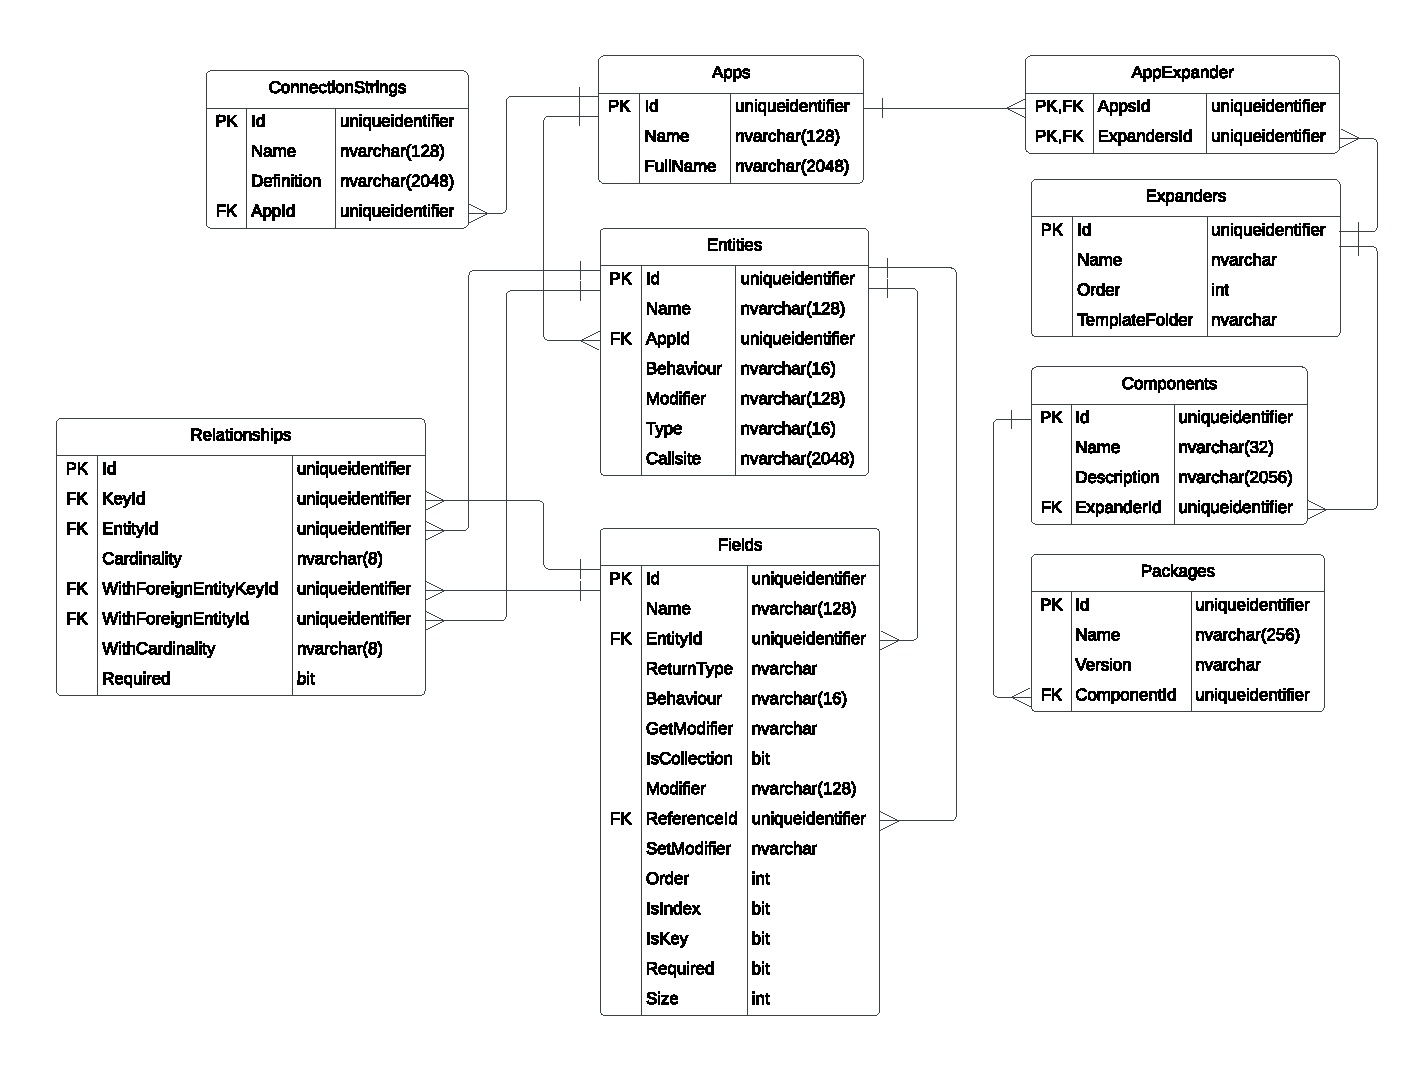
\includegraphics[width=1\textwidth]{figures/erd.pdf}
    \caption[The meta-model represented as an Entity Relationship Diagram]{The meta-model represented as an Entity Relationship Diagram}
    \label{fig_erd}
\end{figure}